%!TEX TS-program = xelatex 
\documentclass[aspectratio=1610,xcolor=dvipsnames,t,compress]{beamer} 

\usepackage{listings} 
\usepackage{color} 
\usepackage{xcolor}  
\usepackage{microtype} 
\usepackage{helvet} 
\usepackage{inconsolata} 
\usepackage[framemethod=TikZ]{mdframed} 
\usepackage{graphicx} 
\usepackage{alltt}
\usepackage{sverb} 
\usepackage{verbatim} 
\usepackage{pifont} 
\usepackage{helvet} 
\usepackage{algorithm}
\usepackage{algpseudocode}

\usetheme[noflama]{sthlm}

%\usetheme{Madrid} 
%\useoutertheme{smoothbars} 
\useinnertheme{rectangles} 

\setbeamertemplate{navigation symbols}{}
\setbeamertemplate{blocks}[default] 

%\definecolor{mypurple}{rgb}{.49,0,98}
%\setbeamercolor*{palette primary}{use=structure,fg=white,bg=green}
%\usecolortheme[rgb={0.9,0.2,0.2}]{structure}
%\usecolortheme[rgb={0.6,0.1,0.1}]{structure}

%\usecolortheme[rgb={0.2, 0.2, 0.8}]{structure} 
\usecolortheme[rgb={0.0, 0.0, 0.8}]{structure} 

\usepackage{color}
\definecolor{orange}{cmyk}{0,0.4,0.8,0.2}
\definecolor{darkorange}{rgb}{.71,0.21,0.01}
\definecolor{darkgreen}{rgb}{.12,.54,.11}
\definecolor{myteal}{rgb}{.26, .44, .56}
\definecolor{gray}{gray}{0.45}
\definecolor{lightgray}{gray}{.95}
\definecolor{mediumgray}{gray}{.8}
\definecolor{inputbackground}{rgb}{.95, .95, .85}
\definecolor{outputbackground}{rgb}{.95, .95, .95}
\definecolor{traceback}{rgb}{1, .95, .95}
\definecolor{inputbg}{rgb}{0.98, 0.98, 0.98}

\usepackage{listings} 
\lstset{language=bash,
        %basicstyle=\footnotesize\ttfamily, 
        basicstyle=\small\ttfamily,
        columns=fullflexible, 
        %title=\lstname, 
        %numbers=left, stringstyle=\texttt, 
        %numberstyle={\tiny\texttt}, 
        keywordstyle=\color{blue}, 
        commentstyle=\color{darkgreen}, 
        stringstyle=\color{purple} } 


\mdfsetup{skipabove=\topskip, skipbelow=\topskip} 

\definecolor{codebg}{rgb}{0.99,0.99,0.99}

\global\mdfdefinestyle{code}{%
    frametitlerule=true,%
    frametitlefont=\small\bfseries\ttfamily,%
    frametitlebackgroundcolor=lightgray,%
    backgroundcolor=codebg,%
    linecolor=gray, linewidth=0.5pt,%
    leftmargin=0.5cm, rightmargin=0.5cm,%
    roundcorner=2pt,%
    innerleftmargin=5pt
}

\global\mdfdefinestyle{code2}{%
    topline=false,%
    bottomline=false,%
    leftline=true,%
    rightline=false,%
    backgroundcolor=codebg,%
    linecolor=gray, linewidth=0.5pt,%
    leftmargin=0.0cm, rightmargin=0.0cm,%
    innerleftmargin=1pt
}

\newcommand{\showcode}[1]{\begin{mdframed}[style=code] %
                            \lstinputlisting{#1}% 
                          \end{mdframed}% 
}

%\title[Software Engineering]{Software Architecture and Architectural Design} 
\title[Software Engineering]{Software Engineering Concepts}
\subtitle{A Brief Introduction} 
\author[Michael Papasimeon]{Dr Michael Papasimeon} 
\date{18 May 2003} 

\begin{document}

\begin{frame}
    \maketitle
\end{frame} 

\begin{frame}{Software Engineering}
    \begin{itemize}
        \item Foundations in System Science and Systems Engineering
        \item The systematic application of science and management to 
              build and deliver software systems with sufficient 
              quality, that satisfy the requirements and are 
              built on time and budget.
        \item Software systems are the most complex systems built by humans. 
        \item Software Engineering aims to manage this complexity.
    \end{itemize}
\end{frame}

\begin{frame}{Lifecycle Phases}
    \begin{itemize}
        \item Business/Domain Modelling 
        \item Requirements
        \item Analysis and Design (Architectural and Detailed)
        \item Implementation (Coding and Integration)
        \item Testing
        \item Deployment
        \item Configuration Management
        \item Project Management
    \end{itemize}
\end{frame}

\begin{frame}{Lifecycle Models}
    \begin{itemize}
        \item Waterfall
        \item Spiral
        \item Agile
        \item Modern software engineering processes are:
            \begin{itemize}
                \item Iterative and incremental
                \item Requirements/functionality driven
                \item Architecture driven (importance of design)
            \end{itemize}
    \end{itemize}
\end{frame} 

\begin{frame}{Failure Rate: Hardware vs Software} 
    \begin{block}{}
        \begin{center} 
        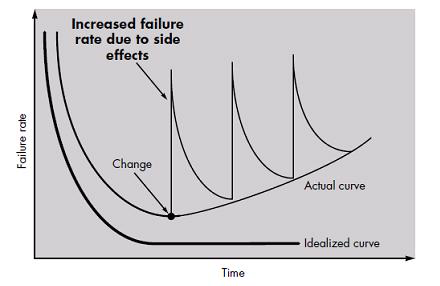
\includegraphics[width=0.6\textwidth]{images/failure-rates} 
        \end{center} 
    \end{block} 
    \tiny{Figure courtesy of \url{http://softwareengineeringhub.blogspot.com.au/2010/03/software-characteristics.html}}
\end{frame} 

\begin{frame}{Impact of Change}
    \begin{itemize}
        \item The later the change in the software lifecycle the greater the
            impact on the project.
        \item Impact may be measured in effort and cost.
        \item For example, there is less impact on the project if a large
            change is needed during the requirements ellicitation phase as
            opposed to the implementation or testing phase. 
    \end{itemize} 
\end{frame}

\begin{frame}{Software Quality Factors} 
    \begin{itemize}
        \item Correctness
        \item Reliability
        \item Robustness
        \item Usability
        \item Efficiency
        \item Modularity
        \item Reusability
        \item Traceability
        \item Maintainability
        \item Extendibility
    \end{itemize}
    \begin{block}{Measuring Software Quality Factors}
        \begin{itemize}
            \item Directly Measurable (e.g. correctness, reliability)
            \item Indirectly Measurable (e.g. usability)
        \end{itemize}
    \end{block} 
\end{frame}

\begin{frame}{Assuring Software Quality} 
    \begin{itemize}
        \item Sofware Engineering Methods
        \item Formal Techncial Reviews
        \item Software Configuration Managment
        \item Software Quality Assurance
        \item Verification and Validation
        \item Standards and Procedures
        \item Testing
    \end{itemize}
\end{frame}

\begin{frame}{Software Reuse} 
    \begin{itemize}
        \item \textbf{Ad-Hoc:} Incidental reuse that occurs through 
              movement of staff through an organisation.
        \item \textbf{Opportunistic:} Organisation taking advantage of reuse 
              opportunities through smart/intelligent design.
          \item \textbf{Integrated:} When opportunities are sought out as 
              part of an organisation’s development process.
          \item \textbf{Leveraged:} Assumes that a given product is part of 
              product family, the members of which have something in common. 
              Construct domains that take in the product family.
          \item \textbf{Anticipated:} Construct domains that anticipate needs
    \end{itemize}
\end{frame} 

\begin{frame}{Coupling and Cohesion} 
    \begin{block}{Inter-Module Coupling} 
        The measure of the interdependence of one module to another. 
        Modules should have low coupling. 
        Low coupling minimizes the "ripple effect" where changes 
        in one module cause errors in other modules. 
    \end{block} 

    \begin{block}{Intra-Module Cohesion} 
        The measure of strength of the association of elements within a module. 
        Modules whose elements are strongly and genuinely related to 
        each other are desired. A module should be highly cohesive. 
    \end{block} 

    \begin{center}
        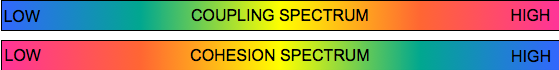
\includegraphics[width=0.7\textwidth]{images/spectra} 
    \end{center}

\end{frame} 

\begin{frame}{Why is Quality Important?}
    The level of quality required depends on the level of impact when risks
    occur.
    \begin{itemize}
        \item Mission Critical Systems
        \begin{itemize}
            \item Safety Critical
            \item Security Critical
        \end{itemize}
        \item Decision Critical Systems 
        \begin{itemize} 
            \item Longer term, safety, security and financial issues
        \end{itemize}
        \item Customer/Financial/Enterprise Critical
        \begin{itemize}
            \item Shorter Term Critical Systems
        \end{itemize} 
    \end{itemize}
\end{frame}

\begin{frame}{Verification and Validation}
    \begin{block}{Verification: “Are we building the system right?”}
        The process of determining that a model implementation accurately 
        represents the developer's conceptual description of the 
        model and the solution to the model. 
    \end{block}

    \begin{block}{Validation: “Are we building the right system?”}
        The process of determining the degree to which a model is an 
        accurate representation of the real world from the 
        perspective of the intended uses of the model. 
    \end{block}

    \begin{block}{Verification and Validation Documentation}
        \begin{itemize}
            \item \textbf{SVVP} Software Verification and Validation Plan
            \item \textbf{SVVR} Software Verificatioi and Validation Report
        \end{itemize}
    \end{block}

\end{frame}

\end{document}
